%\title{LaTeX Portrait Poster Template}
%%%%%%%%%%%%%%%%%%%%%%%%%%%%%%%%%%%%%%%%%
% a0poster Portrait Poster
% LaTeX Template
% Version 1.0 (22/06/13)
%
% The a0poster class was created by:
% Gerlinde Kettl and Matthias Weiser (tex@kettl.de)
% 
% Adapter by Jens Buysse for Hogeschool Gent
% This template has been downloaded from:
% http://www.LaTeXTemplates.com
%
% License:
% CC BY-NC-SA 3.0 (http://creativecommons.org/licenses/by-nc-sa/3.0/)
%
%%%%%%%%%%%%%%%%%%%%%%%%%%%%%%%%%%%%%%%%%

%----------------------------------------------------------------------------------------
%	PACKAGES AND OTHER DOCUMENT CONFIGURATIONS
%----------------------------------------------------------------------------------------

\documentclass[a0,portrait]{a0poster}

\usepackage{multicol} % This is so we can have multiple columns of text side-by-side
\columnsep=100pt % This is the amount of white space between the columns in the poster
\columnseprule=3pt % This is the thickness of the black line between the columns in the poster

\usepackage[svgnames]{xcolor} % Specify colors by their 'svgnames', for a full list of all colors available see here: http://www.latextemplates.com/svgnames-colors

\usepackage{times} % Use the times font
%\usepackage{palatino} % Uncomment to use the Palatino font

\usepackage{graphicx} % Required for including images
\graphicspath{{figures/}} % Location of the graphics files
\usepackage{booktabs} % Top and bottom rules for table
\usepackage[font=small,labelfont=bf]{caption} % Required for specifying captions to tables and figures
\usepackage{amsfonts, amsmath, amsthm, amssymb} % For math fonts, symbols and environments
\usepackage{wrapfig} % Allows wrapping text around tables and figures
\usepackage[export]{adjustbox}

\begin{document}

%----------------------------------------------------------------------------------------
%	POSTER HEADER 
%----------------------------------------------------------------------------------------

% The header is divided into two boxes:
% The first is 75% wide and houses the title, subtitle, names, university/organization and contact information
% The second is 25% wide and houses a logo for your university/organization or a photo of you
% The widths of these boxes can be easily edited to accommodate your content as you see fit

\begin{minipage}[t]{0.75\linewidth}
\VeryHuge \color{HoGentAccent1} \textbf{Docker for Windows} \color{Black}\\ % Title
%\Huge\textit{Ondertitel (eventueel)}\\[2.4cm] % Subtitle
\huge \textbf{Heirbaut Stephan, Schepens Gert, Vermeulen Steven}\\[0.5cm] % Author(s)
\huge Hogeschool Gent, Valentin Vaerwyckweg 1, 9000 Gent\\[0.4cm] % University/organization
\Large \texttt{stephan.heirbaut.w1409@student.hogent.be} \\
\end{minipage}
%
\begin{minipage}[t]{0.25\linewidth}

\includegraphics[width=13cm,right]{figures/HG-woordmerk.jpg} 

\end{minipage}

\vspace{1cm} % A bit of extra whitespace between the header and poster content

%----------------------------------------------------------------------------------------

\begin{multicols}{2} % This is how many columns your poster will be broken into, a portrait poster is generally split into 2 columns

%----------------------------------------------------------------------------------------
%	ABSTRACT
%----------------------------------------------------------------------------------------

\color{HoGentAccent1} % Navy color for the abstract

\begin{abstract}
Docker for Windows Server 2016 is beschikbaar sinds september 2016, maar het heeft nog geen doorbraak gehad bij de DevOps. Dit ondanks het feit dat het een krachtige tool is voor hen, zeker als men ook een Microsoft Certified Partner wil zijn. Het voorstel van deze bachelorproef is om een onderzoek uit te voeren naar hoe krachtig Docker kan zijn op een Windows Server 2016, teneinde zo meer opties te hebben om deze technologie te deployen. Er zal dus een opstelling gebeuren van een Windows Server 2016 en een CentOS server met Docker, waarbij beiden de taak zullen krijgen om dezelfde applicaties te deployen. De verwachting is dat Docker het op beide platformen er even goed van af brengt, maar ook dat er zeker nog werk aan de winkel is op vlak van documentatie. DevOps is namelijk een groeiend principe, en terecht. Hoe meer opties zij dus hebben, hoe beter.
\end{abstract}
%----------------------------------------------------------------------------------------
%	INTRODUCTION
%----------------------------------------------------------------------------------------

\color{HoGentAccent1} 
\section*{Introductie}
\color{black}
\color{black}
Voorheen kon men Docker enkel installeren op Linux servers. Veel keuze had men dus niet wat betreft het OS waarop men het wou deployen. Maar recent werd Docker ook geïntroduceerd voor Windows Server 2016, waarin men handig gebruik maakt van de Hyper-V containers die er ingebouwd in zitten. In de afgelopen 4 jaar waarin Docker op de markt is gekomen, heeft het veel gedaan voor DevOps-teams. Het is dus zeker de moeite waard om eens te kijken of de Hyper-V containers mooi integreren in Docker en hoe dat precies gebeurt. Het doel en de onderzoeksvraag van deze bachelorproef is dus: Hoe vlot werkt Docker op Windows Server 2016, zeker voor het deployen van .Net-applicaties, ten opzichte van Docker voor Linux?
%----------------------------------------------------------------------------------------
%	GEOLOGY
%----------------------------------------------------------------------------------------

\color{Black} % DarkSlateGray color for the rest of the content
\color{HoGentAccent1} 
\section*{Experimenten}
\color{black}

Als eerste werd de gevonden en gebruikte documentatie vergelijken op vlak van volledigheid en bruikbaarheid.

Vervolgens werden er 2 opstellingen opgebouwd, één voor Docker for Windows en één voor Docker for Linux. De installatie van deze omgevingen werden geautomatiseerd door gebruik te maken van Vagrant en scripting talen zodat deze telkens op dezelfde manier geïnstalleerd werden. Zonder variantie van invloed door gebruikersinvoer.

Daarnaast werden beide opstelling getest op snelheid door gebruik te maken van het 'time vagrant up'- en 'time vagrant provision'-commando. Via 'up' mat de benodigde tijd om een volledige installatie uit te voeren. 'provision' mat alleen de benodigde tijd om een container te installeren.

Ten slotte, werd er ook een security review uitgevoerd. Waarbij er gekeken werd naar welke mogelijkheden er waren om beide opstelling te beveiligen dat ze voldoen aan industrie standaarden.

\color{HoGentAccent1} 
\section*{Sectie met figuur}
\color{black}

\begin{center}\vspace{1cm}
	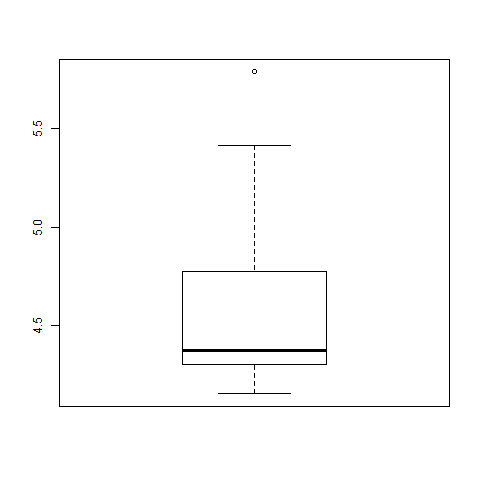
\includegraphics[width=0.4\linewidth]{centosfullboxplot}
	\captionof{figure}{\color{HoGentAccent5} Resultaten benodige voor de volledige installaties van Docker for Linux op CentOS 7.4}
\end{center}\vspace{1cm}

\begin{center}\vspace{1cm}
	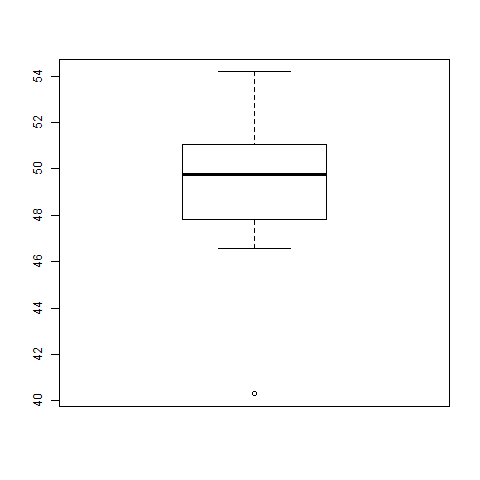
\includegraphics[width=0.4\linewidth]{windowsboxplotfull}
	\captionof{figure}{\color{HoGentAccent5} Resultaten benodige voor de volledige installaties van Docker for Windows op Windows Server 2016}
\end{center}\vspace{1cm}

\begin{center}\vspace{1cm}
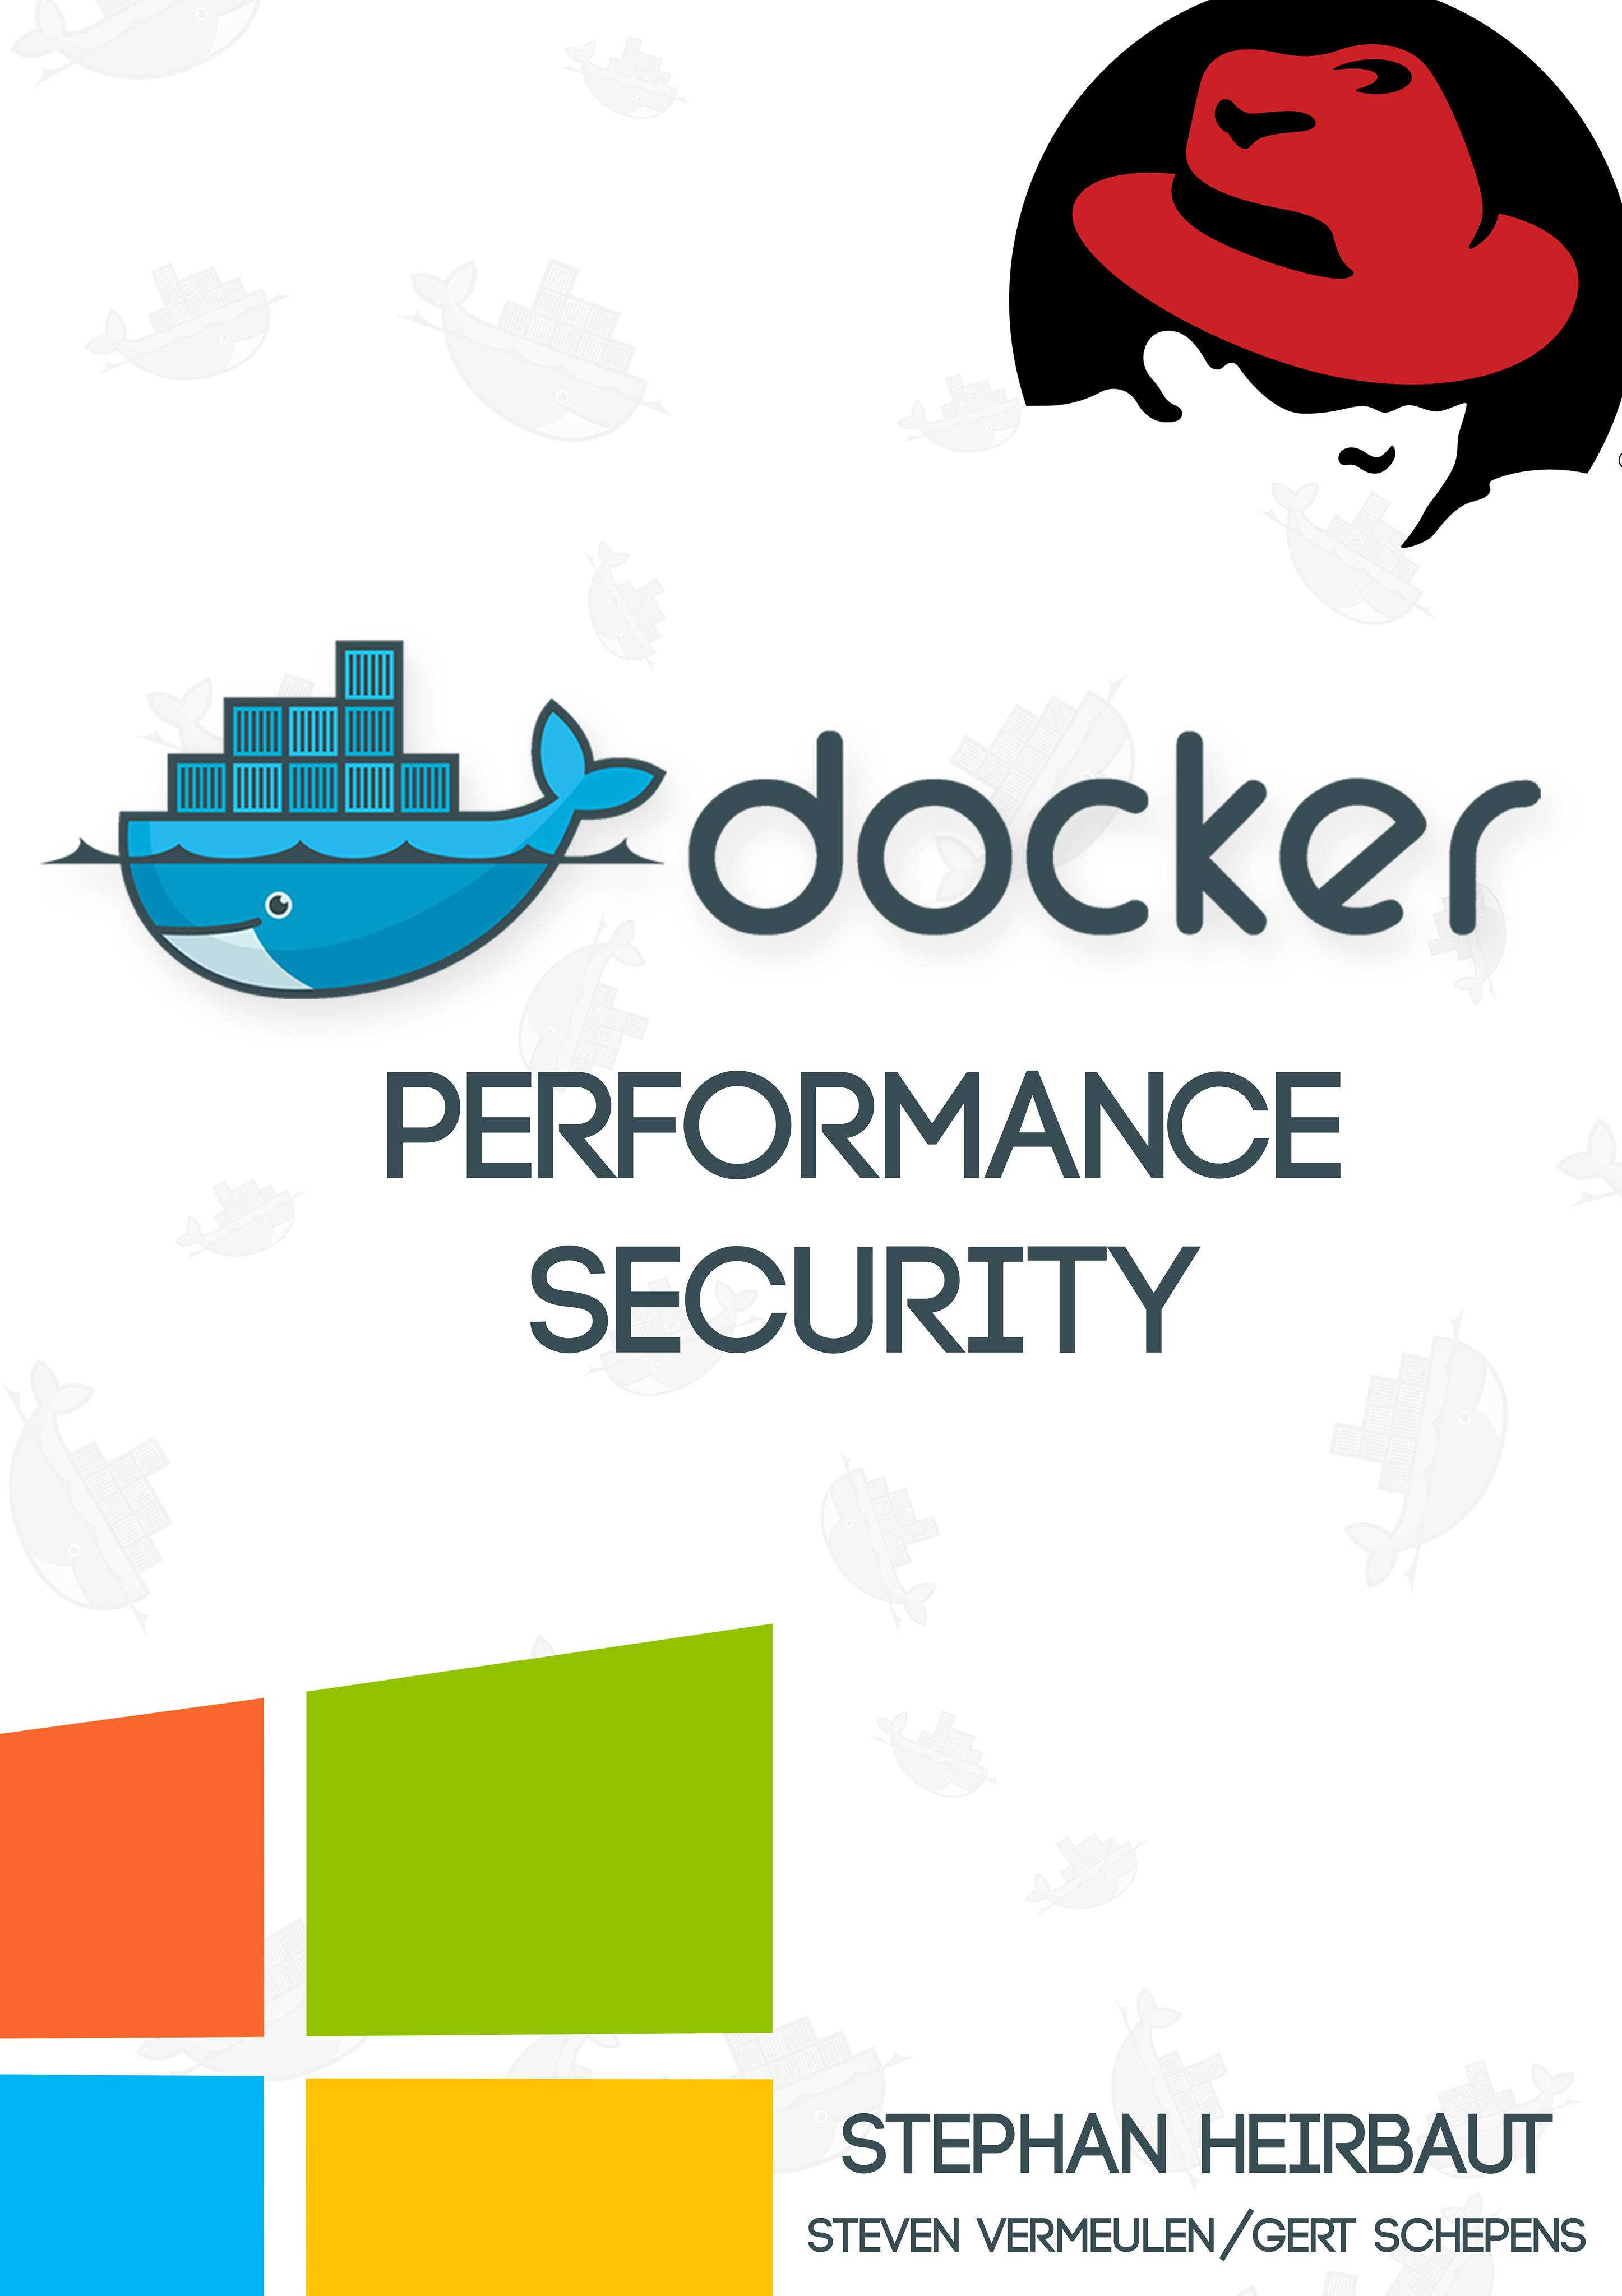
\includegraphics[width=1.0\linewidth]{poster03}
\captionof{figure}{\color{HoGentAccent5} Een vergelijkende studie tussen Docker for Linux en Docker for Windows}
\end{center}\vspace{1cm}

%------------------------------------------------



\color{HoGentAccent1} 
\section*{Conclusies}
\color{black}
De resultaten van dit onderzoek waren min of meer verwacht met enkele interessante ontdekkingen, zoals:
Het grote verschil in benodigde tijd om een installatie van het besturingssysteem en/of container uit te voeren. Dit komt door 3 grote pijnpunten:
\begin{itemize}
	\item Docker CE for Windows vereist een GUI.
	\item Automatisatie is veel moeilijker voor Docker for Windows.
	\item Images en containers zijn groter bij Docker for Windows.
\end{itemize}
Daarnaast zit het qua beveiliging bij beide systemen goed. Voor Docker for Windows vooral omdat Hyper-V containers een extra scheidingslaag heeft tussen de containers en de kernel. Waarbij bij Linux er meer vrijheid is voor de administrator om zelf dingen in te stellen.
Ten slotte, in de context van deze bachelorproef, kan men daarom stellen dat Docker for Linux toch nog steeds beter geschikt is voor DevOps teams of bedrijven die professioneel met containers willen werken. Docker for Windows is wel een geschikte tool voor individuele developers die al op een Windows computer aan het werken zijn.

%----------------------------------------------------------------------------------------
%	FORTHCOMING RESEARCH
%----------------------------------------------------------------------------------------
\color{HoGentAccent1} 
\section*{Toekomstig onderzoek}
\color{black}

Verdere onderzoeksvragen die uit deze bachelorproef oprijzen zijn:
\begin{itemize}
	\item Hoe goed integreert Docker for Linux met het Windows-besturingssysteem?
	\item Kun je de installatie van Docker for Windows beter automatiseren door PowerShell modules aan te maken?
	\item Zijn er manieren om de grootte van de Hyper-V containers te verkleinen?
\end{itemize}

%----------------------------------------------------------------------------------------

\end{multicols}
\end{document}